\chapter{Méthodologie et conception du système}

\section{Introduction}

Ce chapitre présente d'abord la \textbf{méthodologie de développement} (organisation, itérations, gestion de versions), puis la \textbf{conception} : architecture logicielle, machine à états, modélisation UML, conception de la base de données et choix technologiques. Conformément à l'objectif du rapport, chaque choix technique est justifié.

\section{Méthodologie de développement}

\subsection{Démarche itérative et incrémentale}

Le projet a été conduit par itérations successives, chacune livrant un incrément testable :

\begin{enumerate}
    \item \textbf{Socle} : authentification, patients/visites, machine à états transactionnelle, boards ;
    \item \textbf{Enrichissement du parcours (V3)} : phases de soin, orientations, historique de triage, cycle des lits, examens et tâches ;
    \item \textbf{Supervision et ressources (V4)} : SLA, alertes, transferts, relèves, indicateurs de capacité ;
    \item \textbf{Assistance IA} : agents de triage, lits, capacité et documentation, sous supervision.
\end{enumerate}

\subsection{Organisation du travail et jalons}

Chaque incrément est matérialisé par une \textbf{migration SQL versionnée} (nommée \texttt{AAAAMMJJ\_description.sql}), ce qui rend l'évolution du schéma reproductible et auditables. Les jalons sont documentés dans le dépôt (plans, notes de passage de phase, rapports de test).

\subsection{Gestion des versions}

Le code est géré avec Git selon une convention de messages claire. Deux dispositifs garantissent l'hygiène du dépôt :

\begin{itemize}
    \item des \textbf{hooks pre-commit} (scripts locaux) qui bloquent les erreurs évidentes ;
    \item un \textbf{pipeline GitHub Actions} « secret guard » qui échoue si un fichier \texttt{.env} est versionné.
\end{itemize}

\section{Architecture logicielle}

\subsection{Architecture en trois couches}

PICU suit une architecture client-serveur en trois couches :

\begin{enumerate}
    \item \textbf{Présentation} : React~19 + Vite + TailwindCSS (tableaux de bord par rôle) ;
    \item \textbf{Application} : Node.js + Express (API REST + Socket.IO), services métier et middleware ;
    \item \textbf{Données} : PostgreSQL hébergé sur Neon.
\end{enumerate}

\subsection{Organisation des services backend}

Le backend est organisé en couches pour séparer les responsabilités :

\begin{itemize}
    \item \textbf{routes} (\texttt{*Routes.js}) : exposition HTTP, contrôle des capacités, validation d'entrée ;
    \item \textbf{services} (\texttt{*Service.js}) : logique métier transactionnelle (par exemple \texttt{visitService}, \texttt{resourceService}, \texttt{supervisionRulesService}, \texttt{transferRequestService}) ;
    \item \textbf{lib} : utilitaires transverses (par exemple \texttt{careStage}, journalisation d'actions) ;
    \item \textbf{middleware} : authentification (\texttt{authenticateJwt}), autorisation (\texttt{requireRole}, \texttt{requireCapability}) ;
    \item \textbf{ai} : agents, orchestrateur, fournisseur NIM, politiques d'action, observabilité.
\end{itemize}

\subsection{Communication REST et temps réel}

La communication combine des requêtes HTTP REST (JSON) et un canal temps réel \textbf{Socket.IO}. Le serveur diffuse des événements dérivés des transitions de visite (notamment \texttt{visit:status\_changed} et \texttt{queue:updated}) afin que tous les postes se synchronisent sans rechargement.

\begin{figure}[H]
    \centering
    % Image à déposer dans rapport-stage/images/ : architecture_picu.png
    \IfFileExists{images/architecture_picu.png}{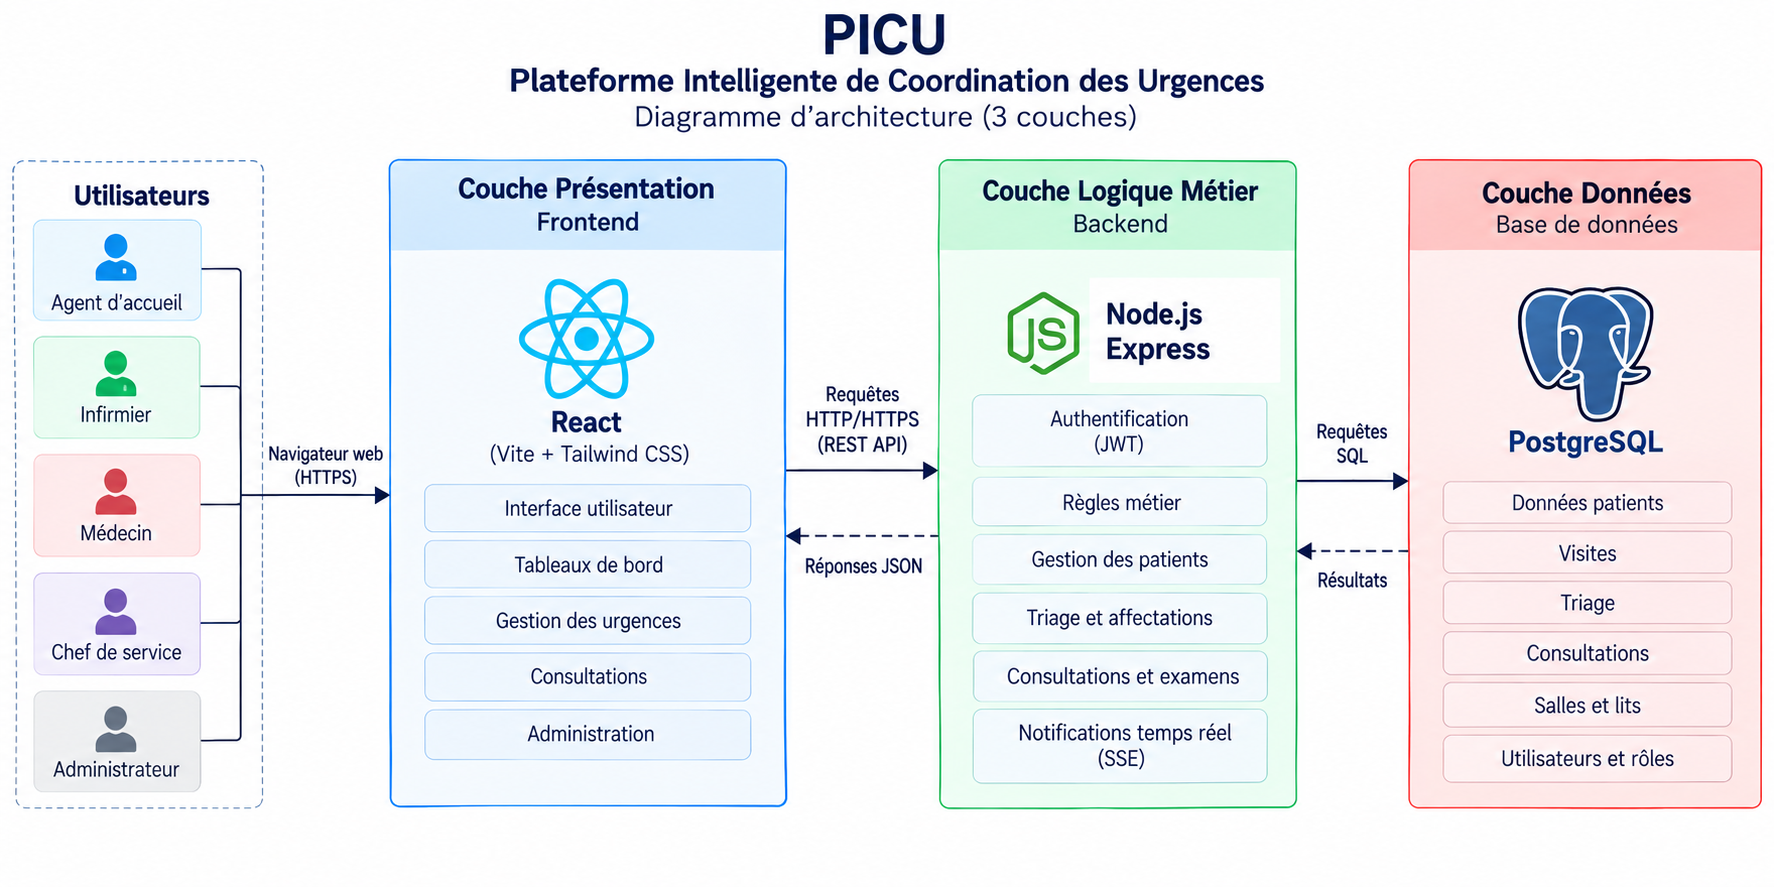
\includegraphics[width=0.92\textwidth]{images/architecture_picu.png}}{\fbox{\parbox{0.92\textwidth}{\centering\vspace{1.5cm}À insérer : \texttt{images/architecture\_picu.png}\vspace{1.5cm}}}}
    \caption{Architecture en trois couches et communications REST/Socket.IO}
    \label{fig:architecture_picu}
\end{figure}

\section{Conception du workflow : machine à états}

\subsection{États de la visite}

Le statut de la visite est la source de vérité du parcours. Il se décompose en trois états principaux et trois états terminaux.

\begin{table}[H]
\centering
\caption{Machine à états du statut de visite}
\label{tab:etats}
\small
\begin{tabular}{|l|l|l|}
\hline
\textbf{Statut} & \textbf{Signification} & \textbf{Transitions sortantes} \\
\hline
\texttt{waiting} & Enregistré, en attente de prise en charge & \texttt{place}, \texttt{close} (parti avant) \\
\hline
\texttt{placed} & Affecté à une ressource & \texttt{start}, \texttt{return}, \texttt{close} \\
\hline
\texttt{in\_treatment} & Prise en charge en cours & \texttt{close} \\
\hline
\texttt{discharged} & Sortie autorisée (terminal) & --- \\
\hline
\texttt{transferred} & Transféré (terminal) & --- \\
\hline
\texttt{left\_without\_seen} & Parti avant prise en charge (terminal) & --- \\
\hline
\end{tabular}
\end{table}

\subsection{Actions et transitions}

Chaque action est une transition atomique exécutée dans une transaction. Le tableau suivant résume les actions autorisées et leurs effets.

\begin{table}[H]
\centering
\caption{Actions de workflow et règles}
\label{tab:actions}
\small
\begin{tabular}{|l|l|l|p{5.4cm}|}
\hline
\textbf{Action} & \textbf{De} & \textbf{Vers} & \textbf{Effet principal} \\
\hline
\texttt{register} & --- & \texttt{waiting} & Crée patient + visite, une seule visite active \\
\hline
\texttt{call} & \texttt{waiting} & \texttt{waiting} & Horodate l'appel, incrémente le compteur \\
\hline
\texttt{place} & \texttt{waiting} & \texttt{placed} & Occupe une ressource libre et compatible \\
\hline
\texttt{return} & \texttt{placed} & \texttt{waiting} & Libère la ressource, remet en file \\
\hline
\texttt{start} & \texttt{placed} & \texttt{in\_treatment} & Ouvre la consultation \\
\hline
\texttt{close} & \texttt{placed}/\texttt{in\_treatment} & terminal & Libère la ressource, fixe l'outcome \\
\hline
\texttt{triage} & \texttt{waiting} & \texttt{waiting} & Enregistre une évaluation de triage \\
\hline
\end{tabular}
\end{table}

\subsection{Dimension multi-états}

Au-delà du statut, la visite porte des dimensions orthogonales qui permettent un suivi fin : la \textbf{phase de soin} (\texttt{care\_stage} : \texttt{registered}, \texttt{triage\_pending}, \texttt{waiting\_care}, \texttt{in\_care}, \texttt{in\_observation}, \texttt{disposition\_pending}, \texttt{completed}), l'\textbf{orientation} (\texttt{critical}, \texttt{acute}, \texttt{standard}, \texttt{ambulatory}, \texttt{observation}, \texttt{isolation}), la \textbf{localisation} du patient et le \textbf{code public}.

\subsection{Conception de la concurrence}

Le point critique est l'affectation des ressources. La solution retenue combine :

\begin{enumerate}
    \item un verrou de ligne sur la visite (\texttt{SELECT ... FOR UPDATE}) ;
    \item une vérification qu'aucune affectation active n'existe pour la ressource ni pour la visite ;
    \item une insertion d'affectation et une mise à jour de statut dans la \textbf{même transaction}.
\end{enumerate}

Ainsi, deux infirmiers qui tentent d'affecter le même lit simultanément voient l'un réussir et l'autre échouer avec un conflit (HTTP~409), sans jamais produire d'état incohérent.

\section{Diagrammes UML}

\subsection{Diagramme de séquence — enregistrement}

\begin{figure}[H]
    \centering
    % Image à déposer dans rapport-stage/images/ : sequence_diagram.png
    \IfFileExists{images/sequence_diagram.png}{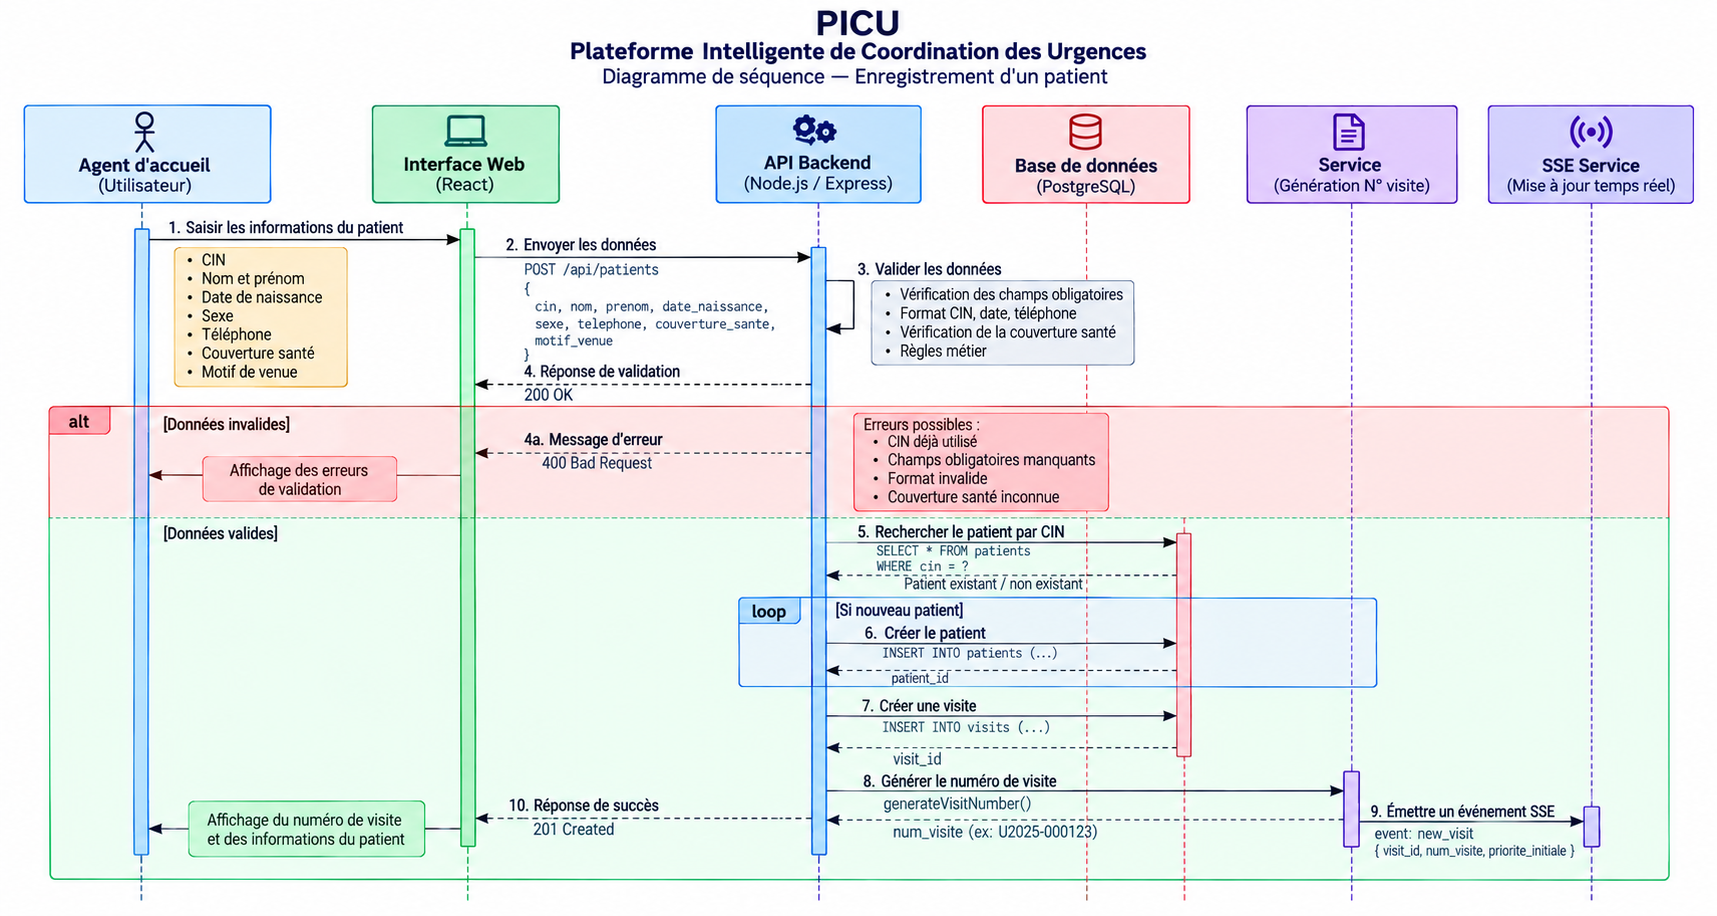
\includegraphics[width=0.9\textwidth]{images/sequence_diagram.png}}{\fbox{\parbox{0.9\textwidth}{\centering\vspace{1.5cm}À insérer : \texttt{images/sequence\_diagram.png}\vspace{1.5cm}}}}
    \caption{Diagramme de séquence — Enregistrement d'un patient}
    \label{fig:sequence_diagram}
\end{figure}

\subsection{Diagramme d'activité — circuit de triage}

\begin{figure}[H]
    \centering
    % Image à déposer dans rapport-stage/images/ : activity_diagram.png
    \IfFileExists{images/activity_diagram.png}{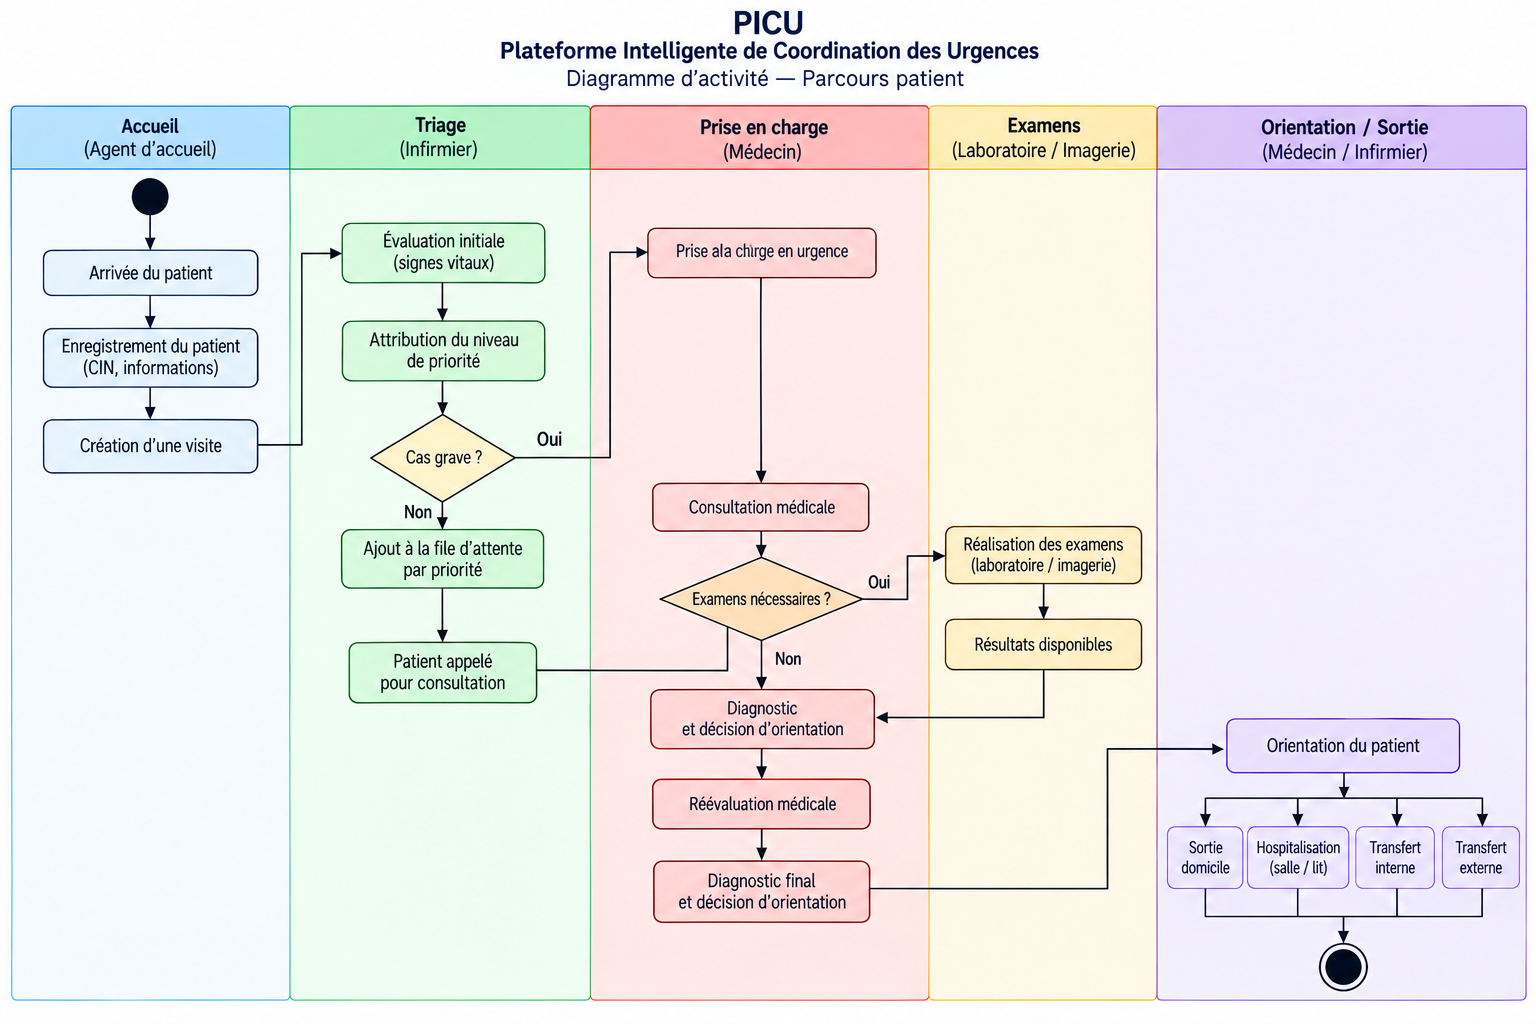
\includegraphics[width=0.9\textwidth]{images/activity_diagram.png}}{\fbox{\parbox{0.9\textwidth}{\centering\vspace{1.5cm}À insérer : \texttt{images/activity\_diagram.png}\vspace{1.5cm}}}}
    \caption{Diagramme d'activité — Circuit de triage et de prise en charge}
    \label{fig:activity_diagram}
\end{figure}

\subsection{Diagramme de classes}

\begin{figure}[H]
    \centering
    % Image à déposer dans rapport-stage/images/ : class_diagram.png
    \IfFileExists{images/class_diagram.png}{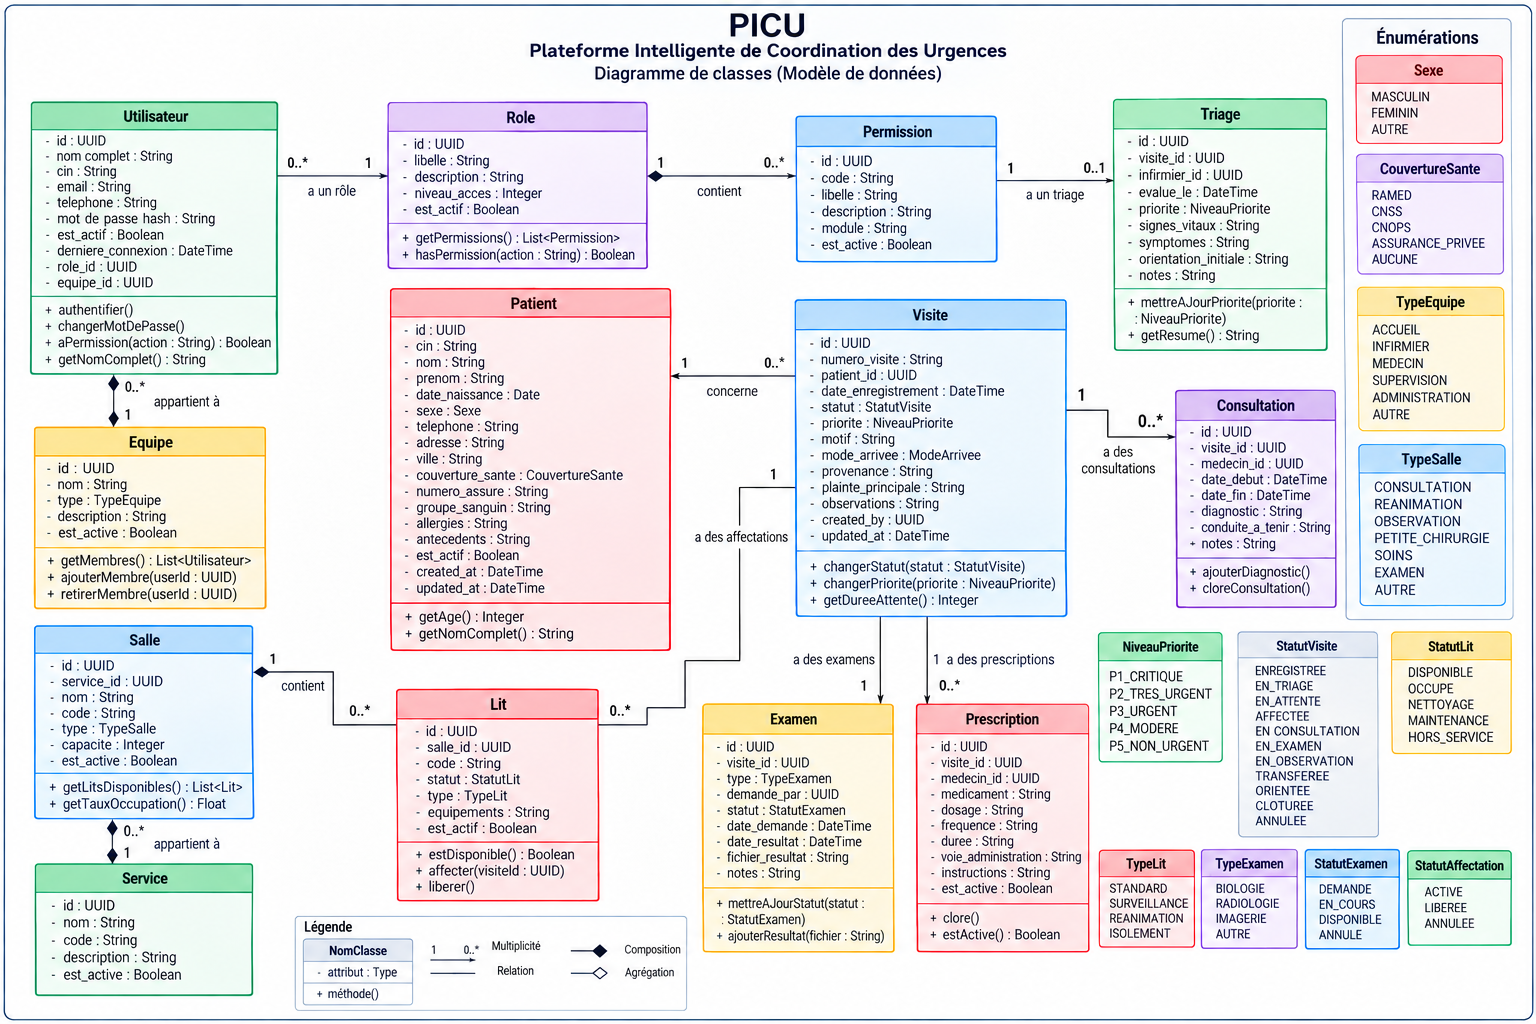
\includegraphics[width=0.9\textwidth]{images/class_diagram.png}}{\fbox{\parbox{0.9\textwidth}{\centering\vspace{1.5cm}À insérer : \texttt{images/class\_diagram.png}\vspace{1.5cm}}}}
    \caption{Diagramme de classes de PICU}
    \label{fig:class_diagram}
\end{figure}

\section{Conception de la base de données}

\subsection{Modèle relationnel}

La base repose sur un schéma relationnel normalisé (3FN). Les entités principales sont : \texttt{users}, \texttt{patients}, \texttt{visits}, \texttt{zones}, \texttt{rooms}, \texttt{beds}, \texttt{bed\_assignments}, \texttt{consultations}, \texttt{triage\_assessments}, \texttt{exams}, \texttt{care\_tasks}, \texttt{visit\_events}, \texttt{room\_teams}, \texttt{resource\_status\_events}, ainsi que les tables V4 (\texttt{transfer\_requests}, \texttt{handoff\_requests}, \texttt{operational\_alerts}, \texttt{workflow\_settings}) et IA (\texttt{agent\_runs}, \texttt{agent\_recommendations}, \texttt{agent\_actions}, \texttt{agent\_approvals}).

\subsection{Contraintes d'intégrité}

L'intégrité est assurée au niveau du schéma par :

\begin{itemize}
    \item des \textbf{clés étrangères} avec politiques de suppression restrictives pour les entités critiques ;
    \item des \textbf{contraintes de domaine} (\texttt{CHECK}) sur les statuts, phases, orientations, outcomes et statuts opérationnels ;
    \item des \textbf{index uniques} empêchant un doublon de code public ou d'affectation active ;
    \item des \textbf{vues} (\texttt{waiting\_board}, \texttt{bed\_board}) exposant l'état consolidé.
\end{itemize}

\subsection{Dictionnaire de données (extrait)}

\begin{table}[H]
\centering
\caption{Dictionnaire de données — extrait}
\label{tab:data_dictionary}
\small
\begin{tabular}{|l|l|p{6cm}|}
\hline
\textbf{Table} & \textbf{Colonne} & \textbf{Description} \\
\hline
visit\_events & event\_type & Type d'événement (enregistré, appelé, placé, triage, clôturé...) \\
\hline
 & actor\_type & \texttt{user}, \texttt{agent} ou \texttt{system} \\
\hline
 & idempotency\_key & Clé unique garantissant la non-duplication d'une action \\
\hline
visits & status & Statut de la machine à états \\
\hline
 & care\_stage & Phase de soin \\
\hline
 & current\_orientation & Orientation clinique courante \\
\hline
beds & resource\_type \texttt{/} operational\_status & Type (lit, fauteuil, box...) et état opérationnel \\
\hline
triage\_assessments & assessment\_type & \texttt{initial}, \texttt{reassessment} ou \texttt{escalation} \\
\hline
transfer\_requests & status & \texttt{pending}, \texttt{confirmed}, \texttt{cancelled}, \texttt{expired} \\
\hline
agent\_actions & requires\_approval & Indique si l'action IA doit être approuvée \\
\hline
\end{tabular}
\end{table}

\subsection{Stratégie de migration}

Chaque évolution est apportée par une migration additive et idempotente (\texttt{ADD COLUMN IF NOT EXISTS}, \texttt{CREATE TABLE IF NOT EXISTS}) appliquée par un script dédié (\texttt{npm run migrate:v3}, \texttt{migrate:v4}, \texttt{migrate:ai}). Cette stratégie permet de faire évoluer un schéma en production sans rupture.

\section{Choix technologiques et justification}

\begin{table}[H]
\centering
\caption{Choix technologiques et justification}
\label{tab:choix}
\small
\begin{tabular}{|l|l|p{6.4cm}|}
\hline
\textbf{Brique} & \textbf{Technologie} & \textbf{Justification} \\
\hline
Frontend & React 19 + Vite & Écosystème mature, composants réutilisables, build rapide. \\
\hline
Style & TailwindCSS & Cohérence visuelle et rapidité de prototypage. \\
\hline
Backend & Node.js + Express & Même langage que le frontend, middleware simple. \\
\hline
Base & PostgreSQL (Neon) & Intégrité relationnelle, transactions, JSONB, gestion managée. \\
\hline
Temps réel & Socket.IO & Diffusion d'événements, repli polling. \\
\hline
Auth & JWT + bcrypt & Standard, sans session serveur. \\
\hline
IA & NVIDIA NIM & Modèles spécialisés, sorties structurées (JSON schema). \\
\hline
\end{tabular}
\end{table}

\section{Conclusion}

La méthode itérative, une architecture en couches, une machine à états explicite et une base fortement contrainte constituent le socle de PICU. Le chapitre suivant détaille la réalisation concrète de ces choix.
